\section{Análisis exploratorio de los datasets}

En esta sección se presenta un análisis preliminar de los datasets utilizados en los experimentos. El objetivo fue examinar sus principales características estructurales y, en particular, el grado de desbalance entre clases, dado que las técnicas de sobremuestreo aplicadas requieren conocer la proporción entre clases mayoritaria y minoritaria para calibrar adecuadamente la generación de instancias sintéticas.

\begin{table}[H]
\centering
\caption{Resumen estadístico de los datasets utilizados}
\begin{tabularx}{\textwidth}{lccccc}
\toprule
\textbf{Dataset} & \textbf{Instancias} & \textbf{Atributos} & \textbf{Clases} & \textbf{Clase minoritaria (\%)} & \textbf{Tipo} \\
\midrule
Breast Cancer & 569 & 30 & 2 & 37.3\% & Binario \\
Ecoli & 336 & 7 & 8 & 0.6\% & Multiclase \\
Glass & 214 & 9 & 6 & 4.2\% & Multiclase \\
Heart Disease & 303 & 13 & 5 & 4.3\% & Multiclase \\
EuroSAT & 27,000 & 13 & 10 & 7.4\% & Imagen \\
\bottomrule
\end{tabularx}
\label{tab:resumen_datasets}
\end{table}

\begin{figure}[H]
\centering

\begin{subfigure}[t]{0.45\textwidth}
  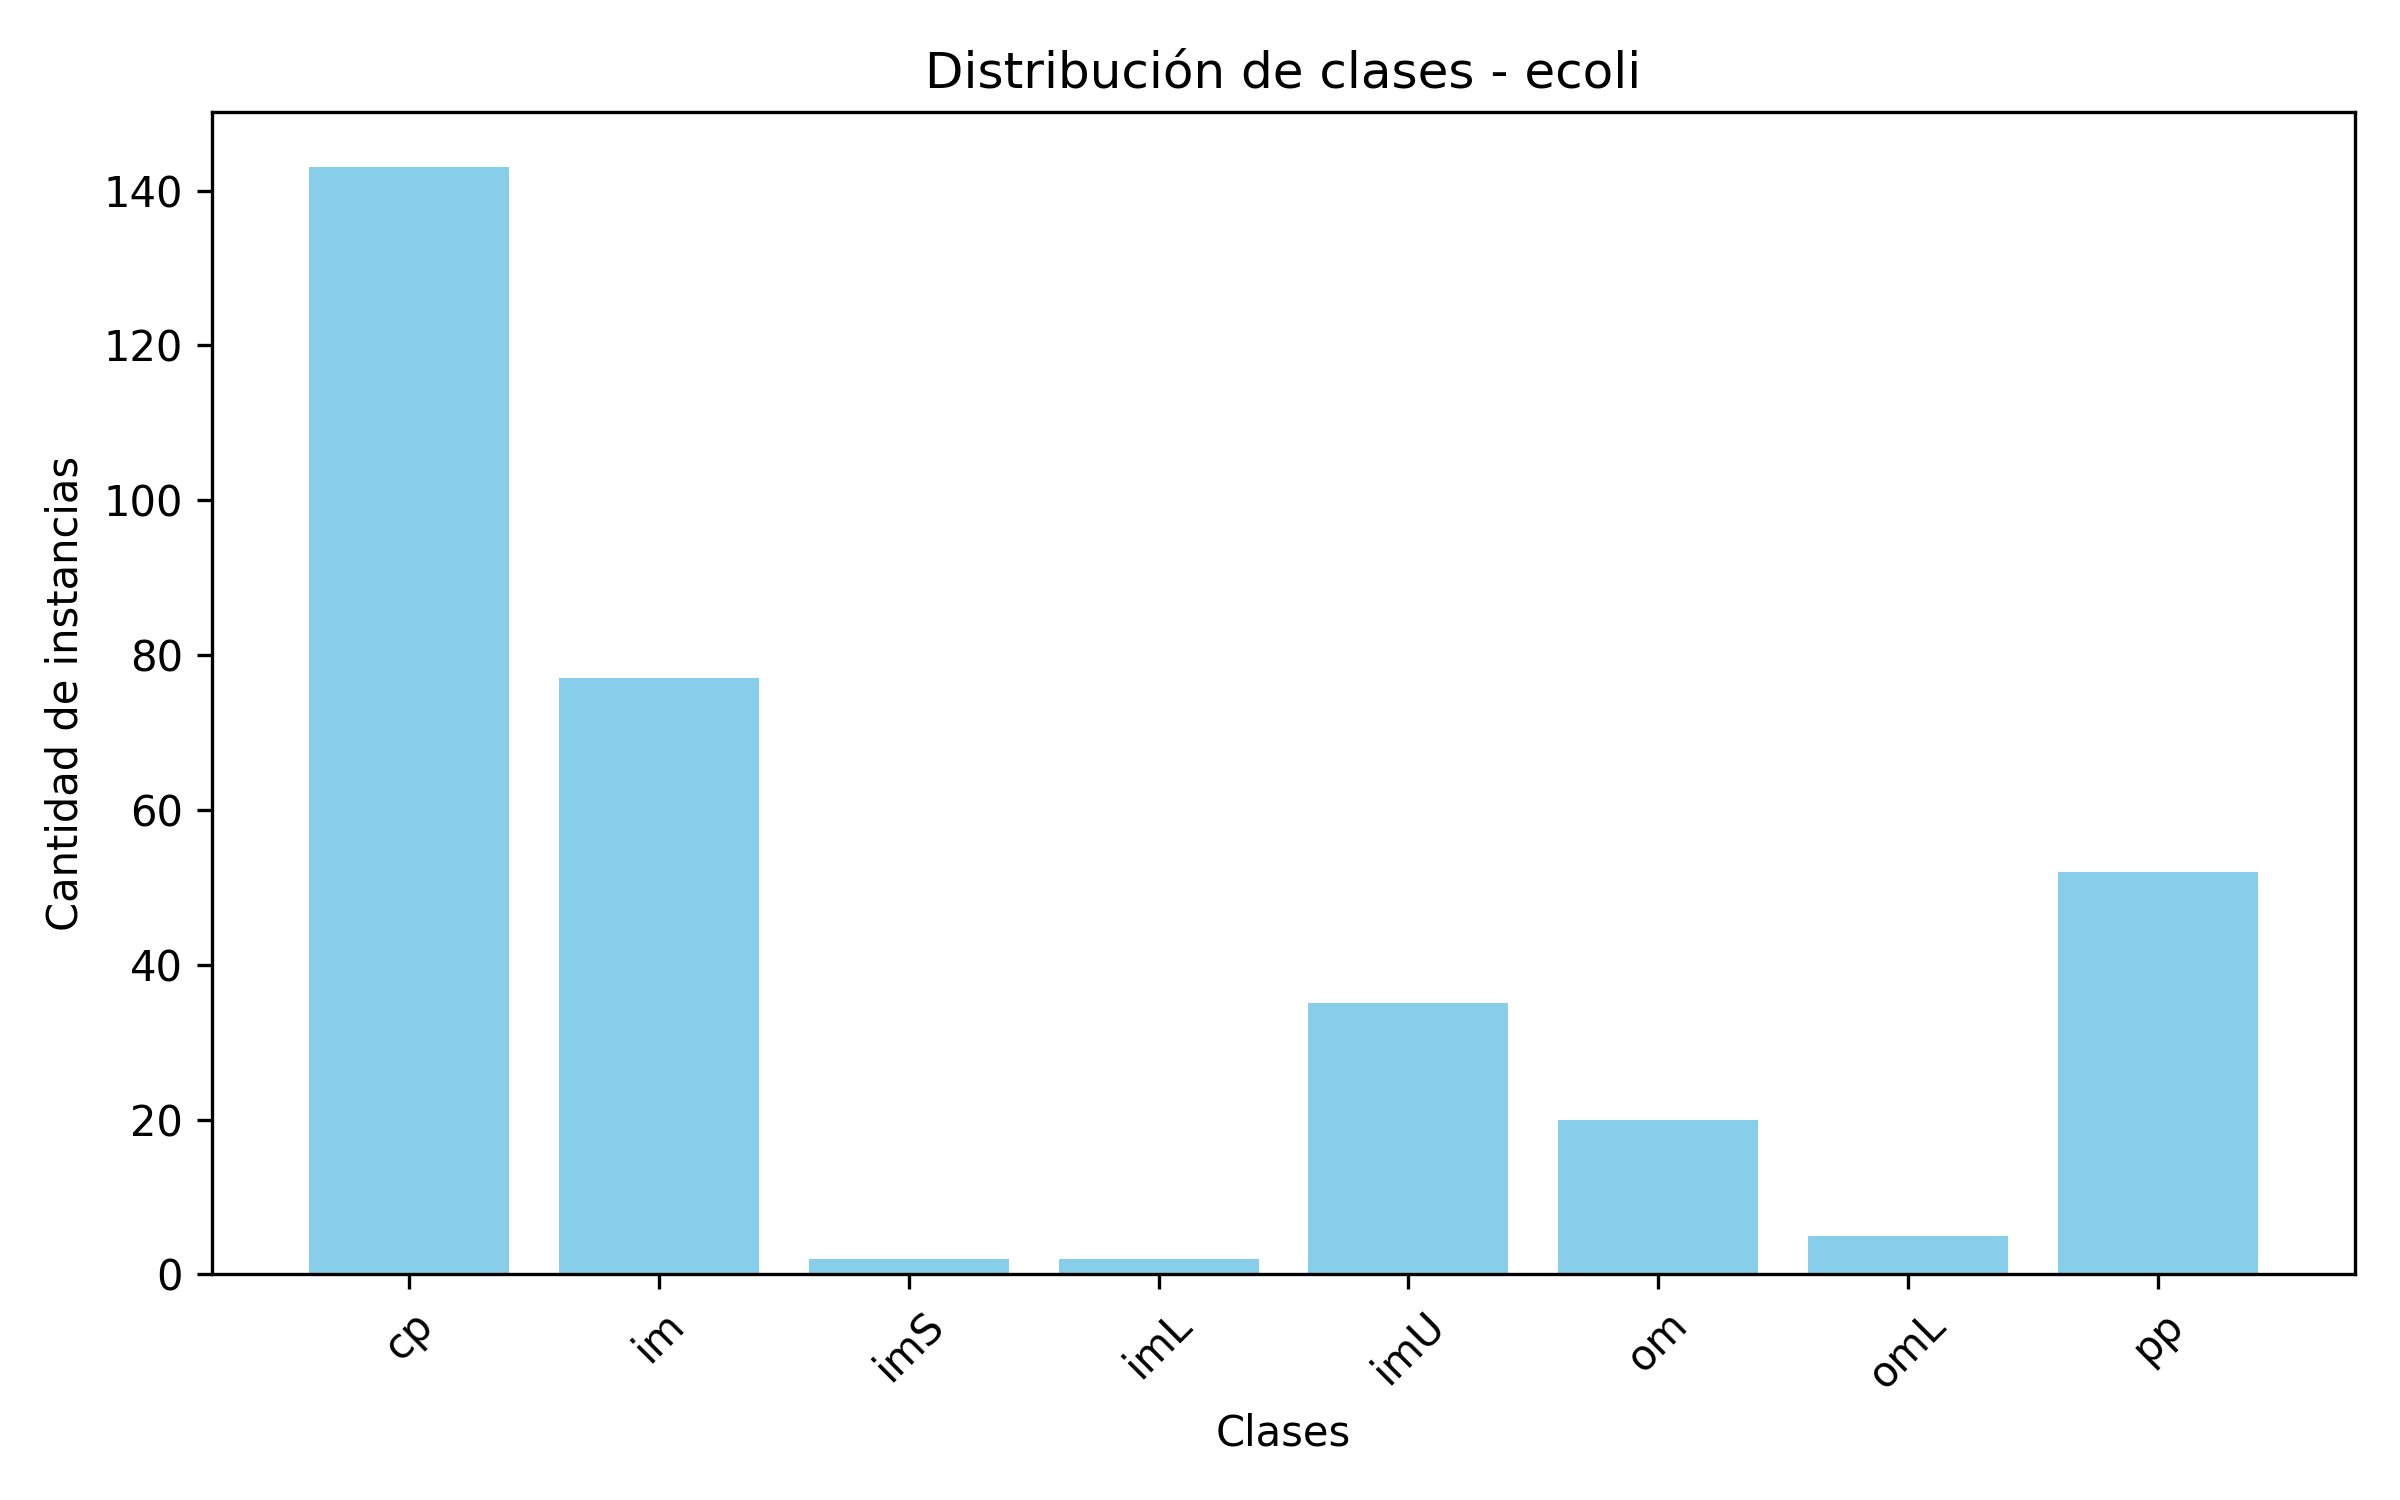
\includegraphics[width=\textwidth]{ecoli_distribucion_2025-07-17_1558.png}
  \caption{Ecoli}
\end{subfigure}
\hfill
\begin{subfigure}[t]{0.45\textwidth}
  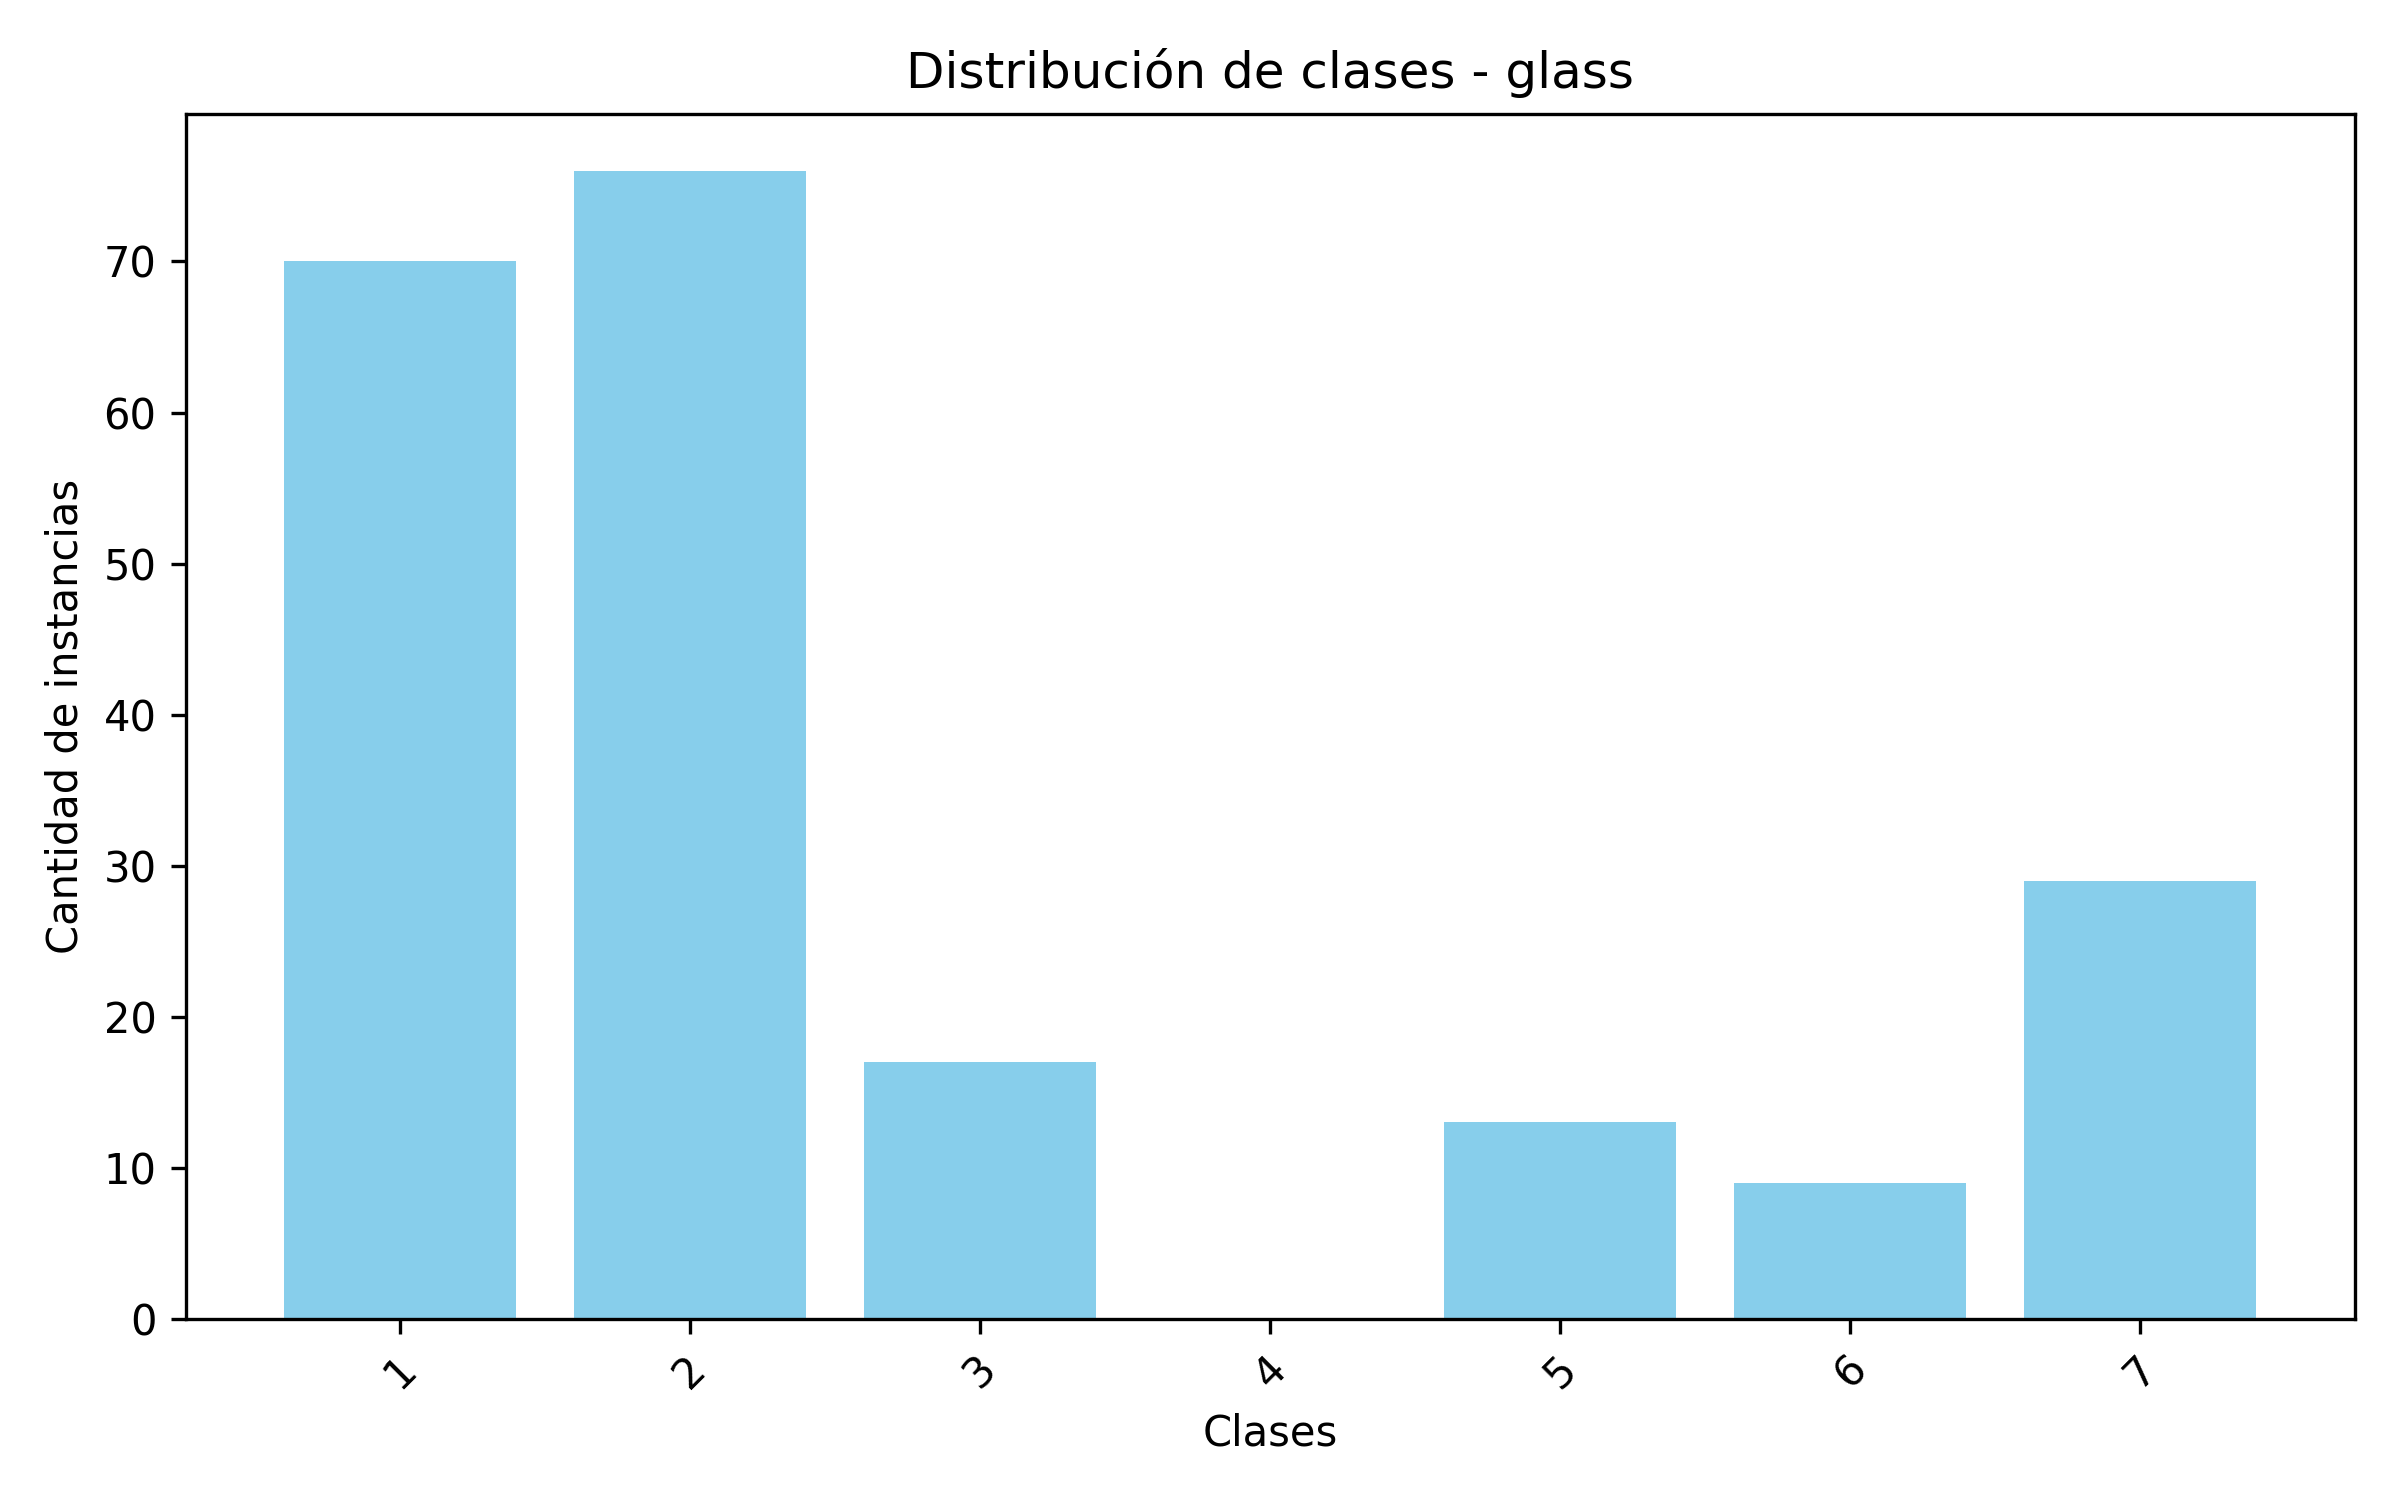
\includegraphics[width=\textwidth]{glass_distribucion_2025-07-17_1558.png}
  \caption{Glass}
\end{subfigure}
\hfill
\begin{subfigure}[t]{0.45\textwidth}
  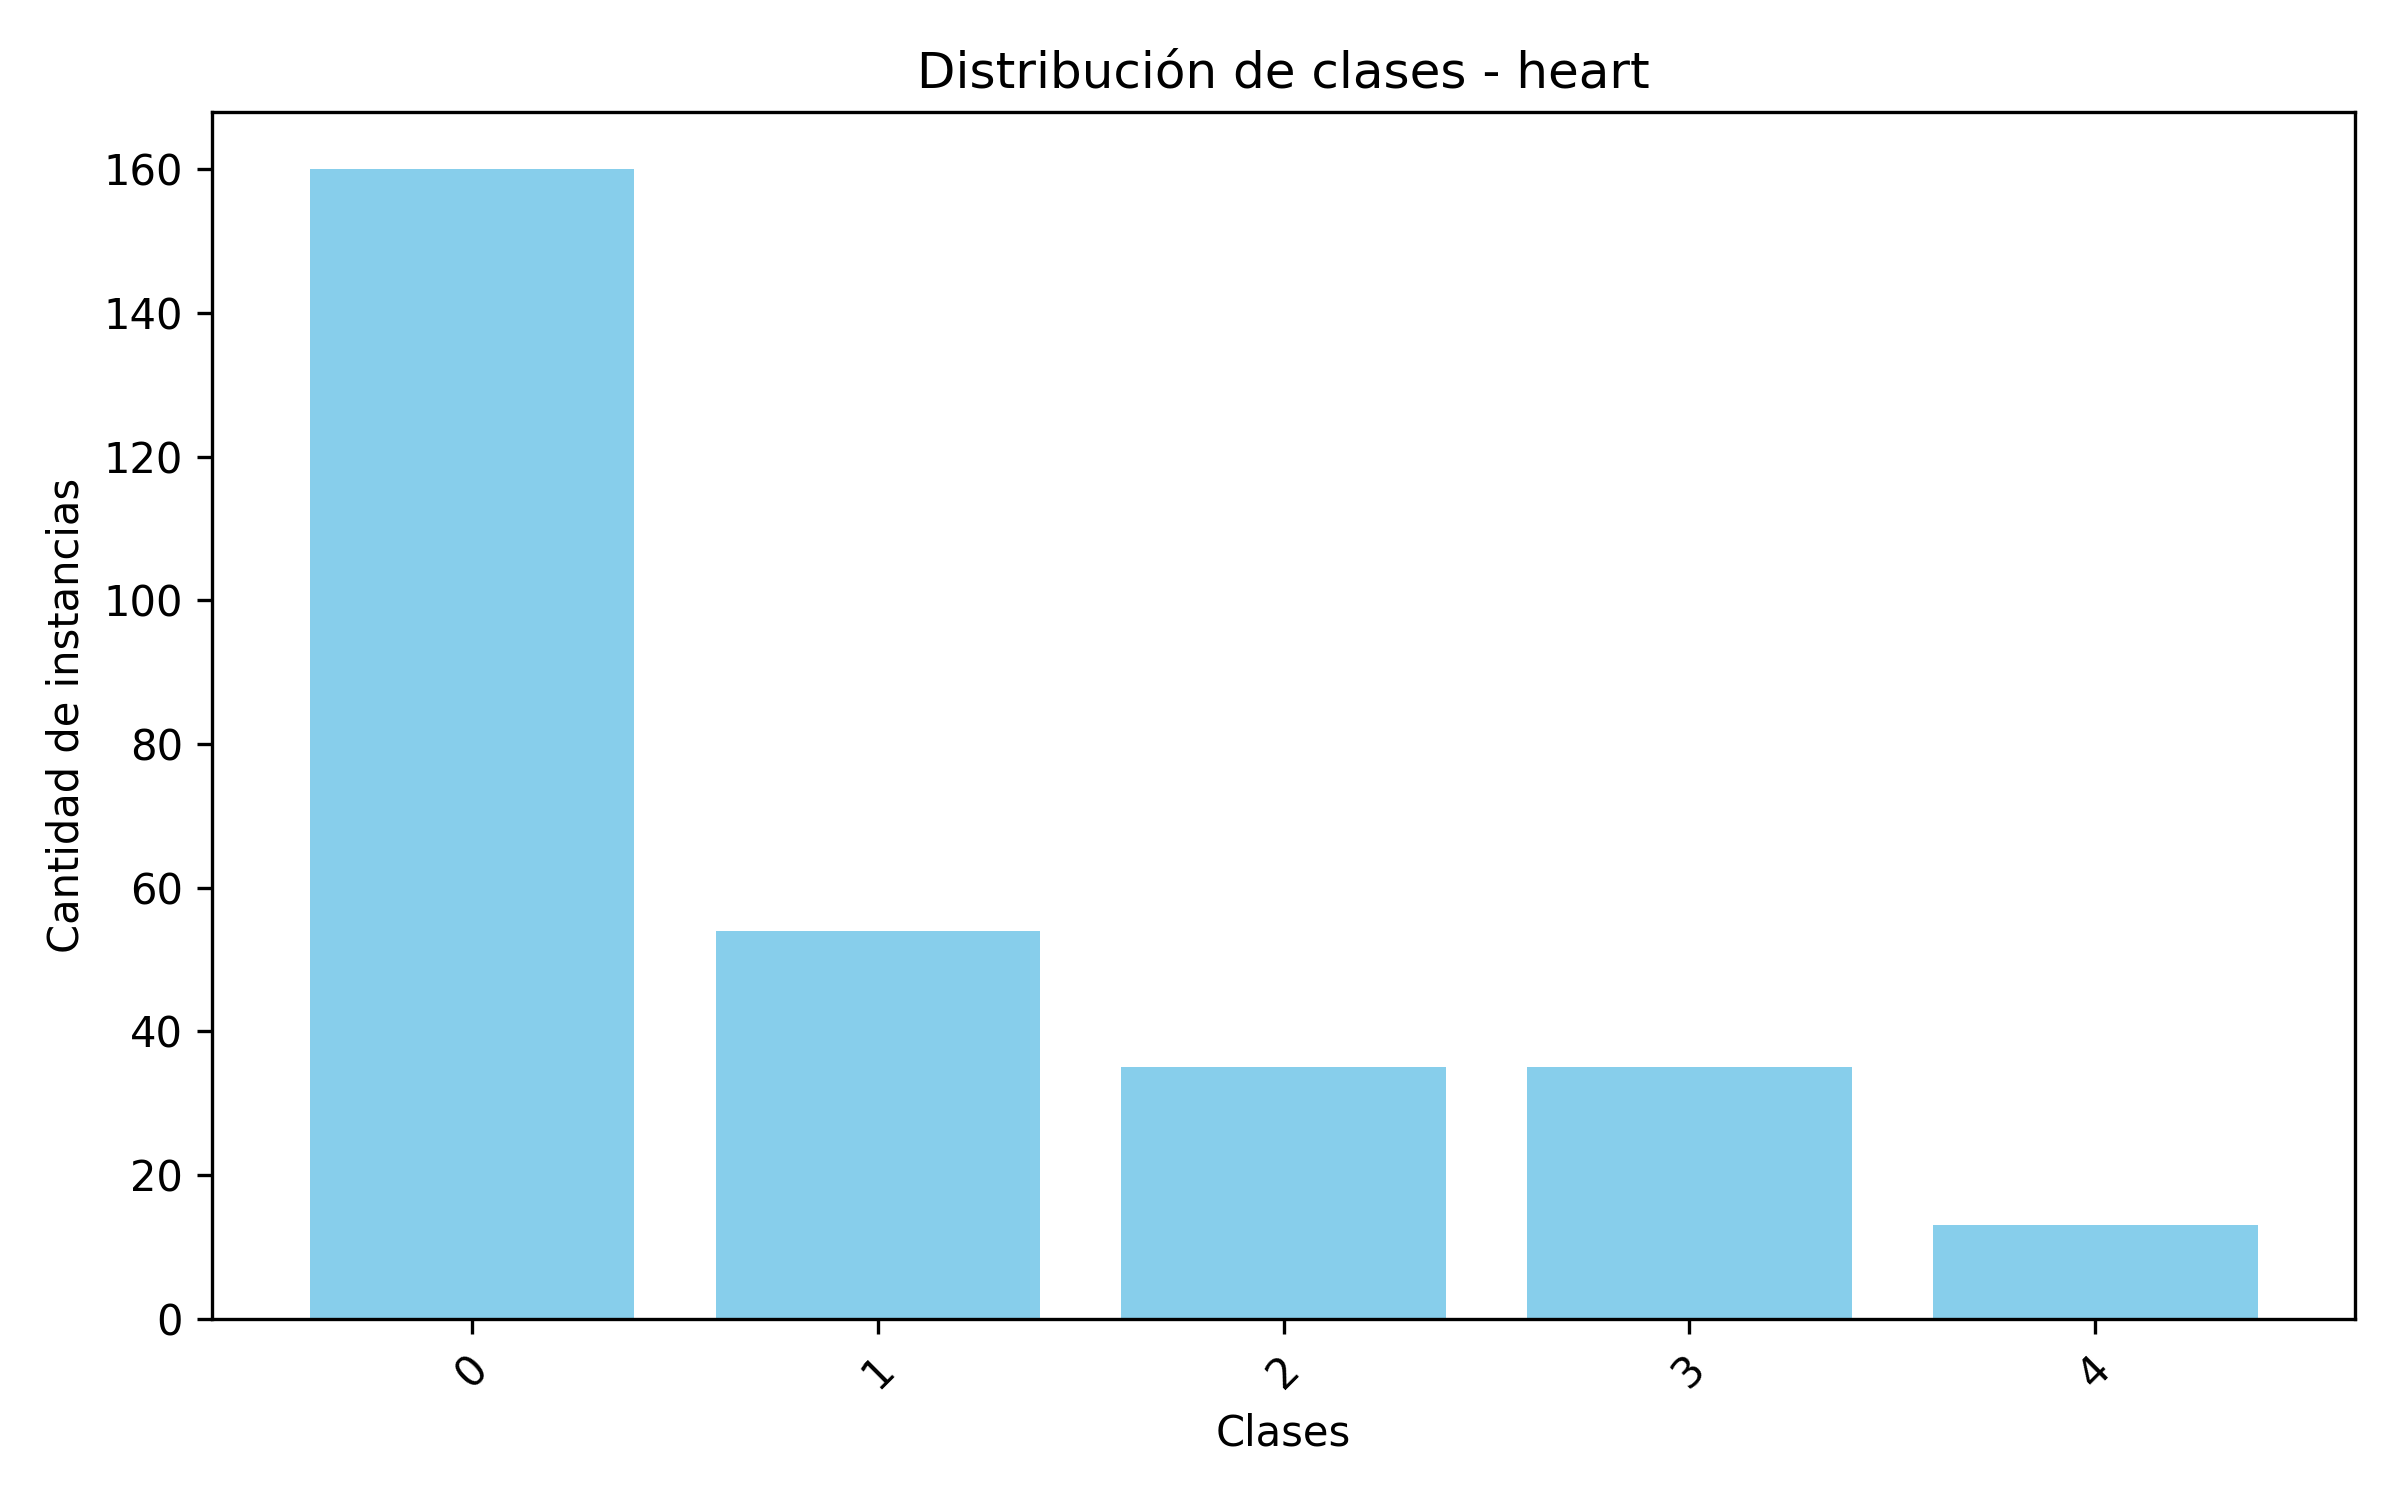
\includegraphics[width=\textwidth]{heart_distribucion_2025-07-17_1558.png}
  \caption{Heart Disease}
\end{subfigure}

\vspace{0.5cm}

\begin{subfigure}[t]{0.45\textwidth}
  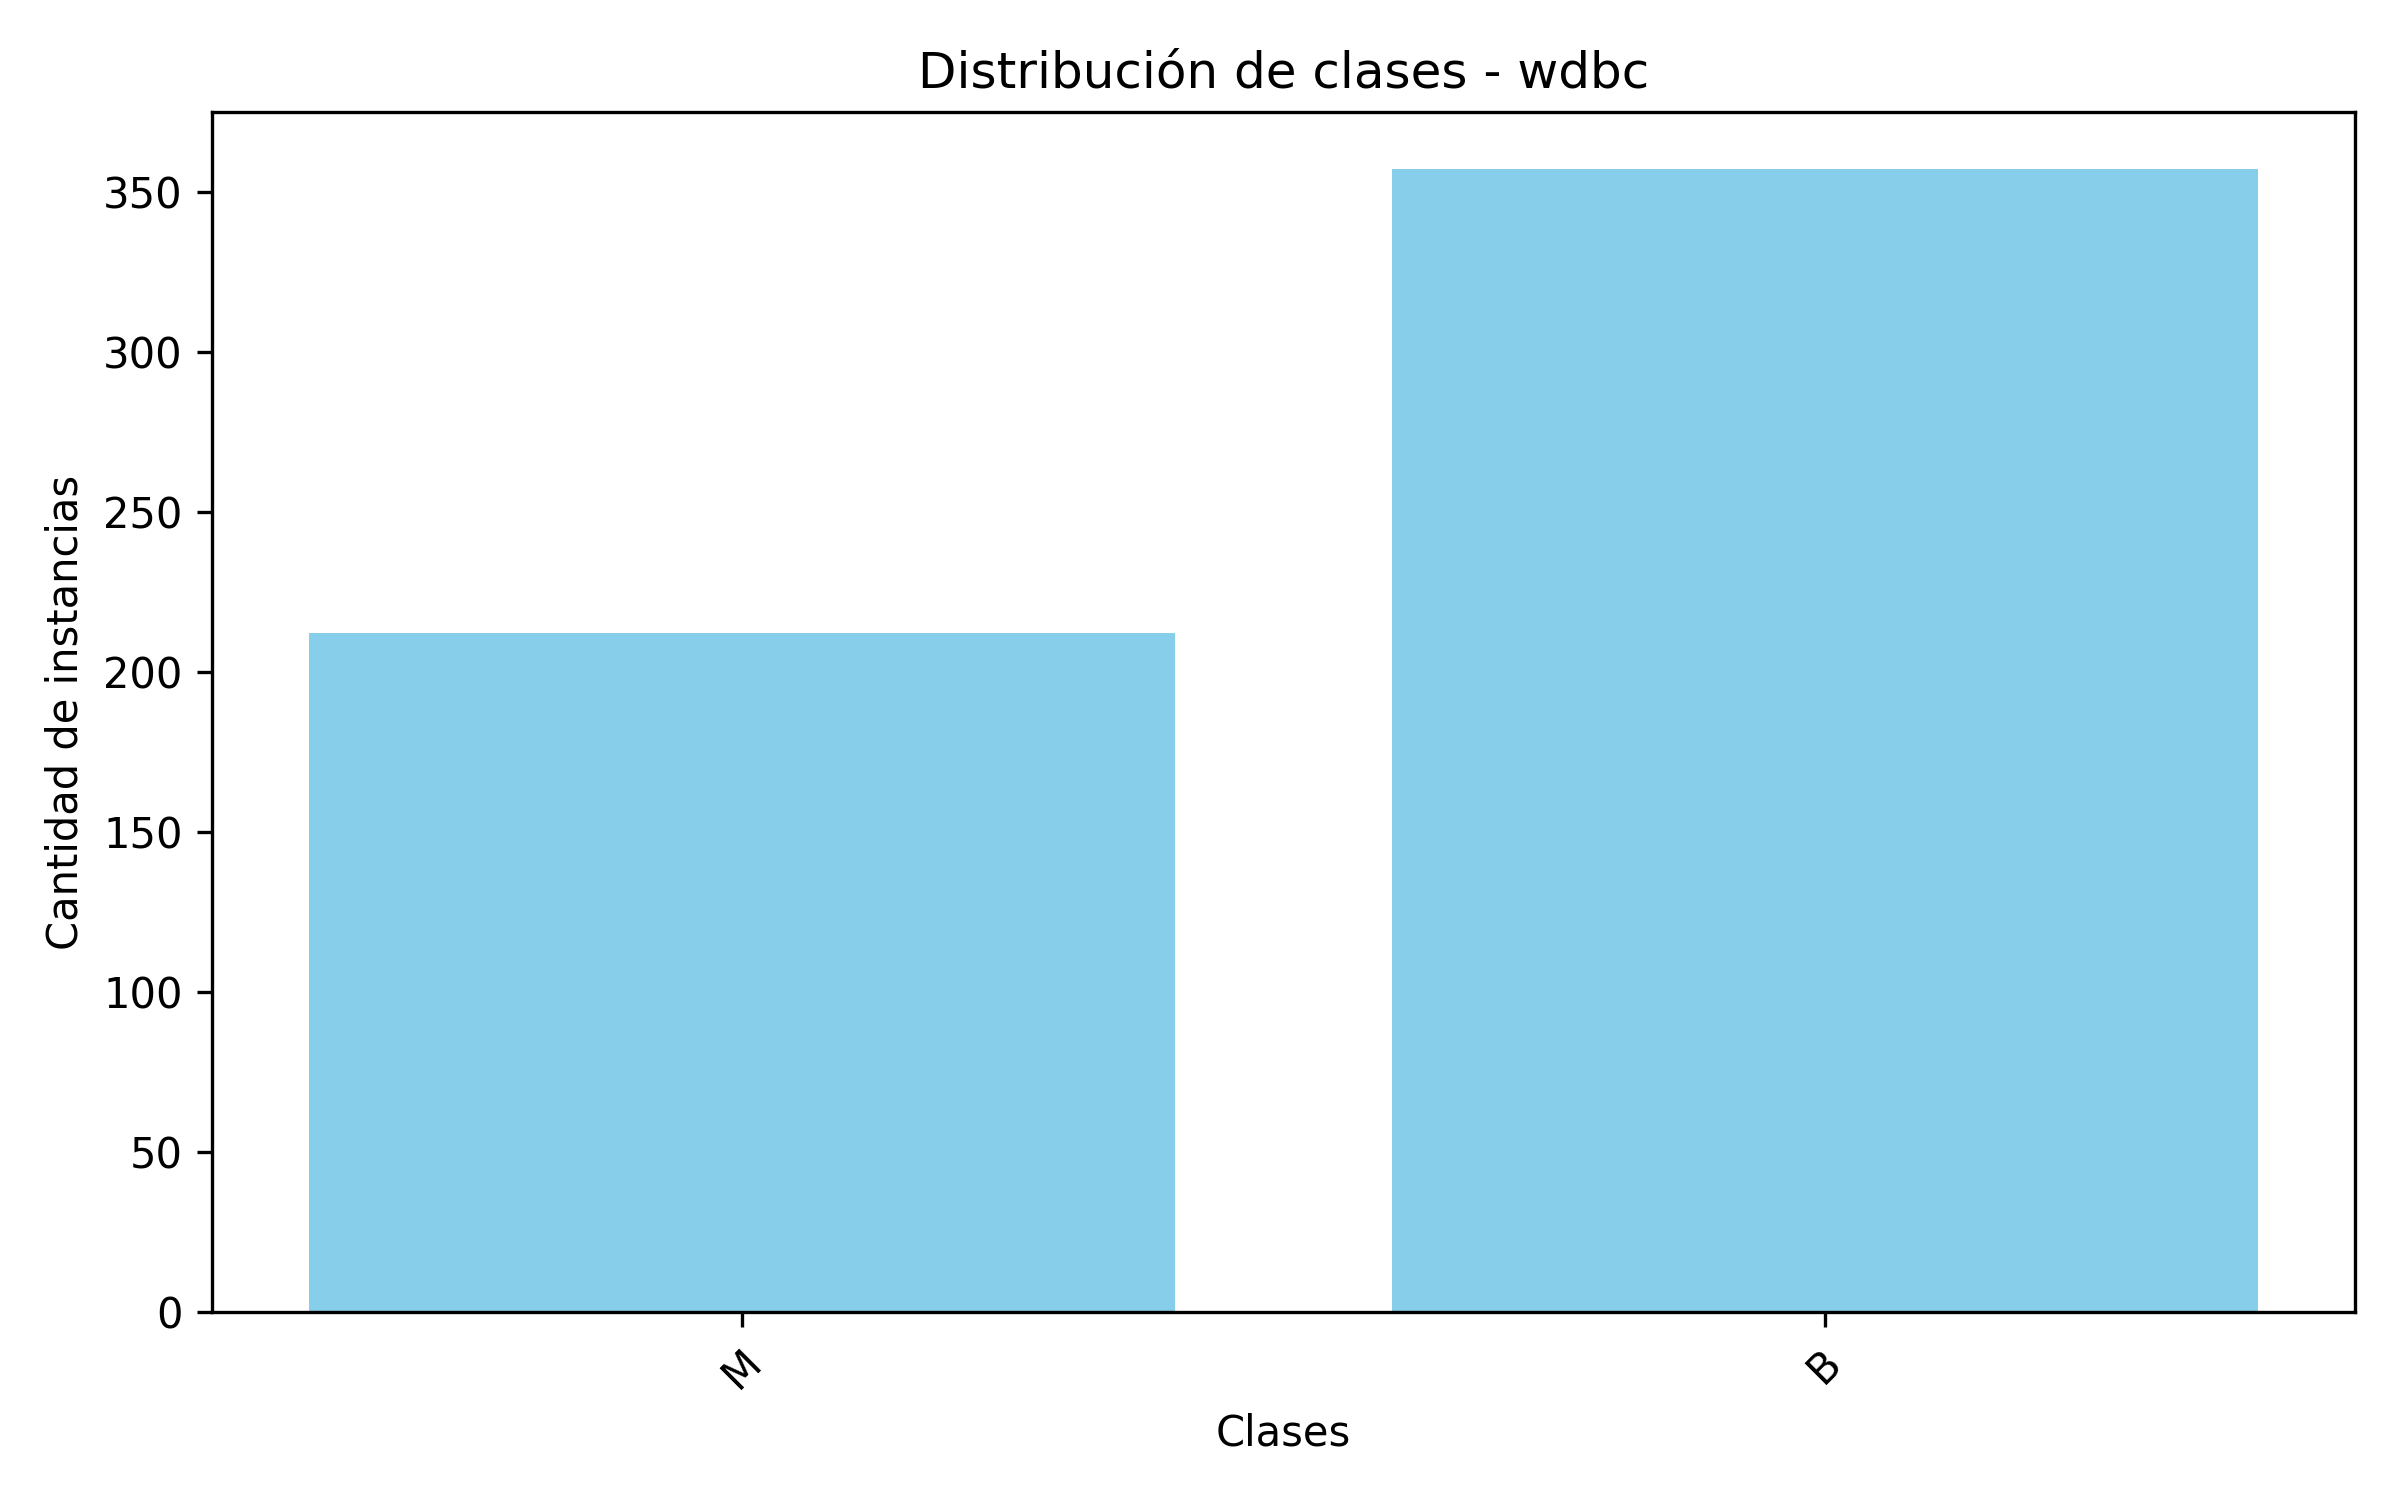
\includegraphics[width=\textwidth]{wdbc_distribucion_2025-07-17_1558.png}
  \caption{Breast Cancer (WDBC)}
\end{subfigure}
\hfill
\begin{subfigure}[t]{0.45\textwidth}
  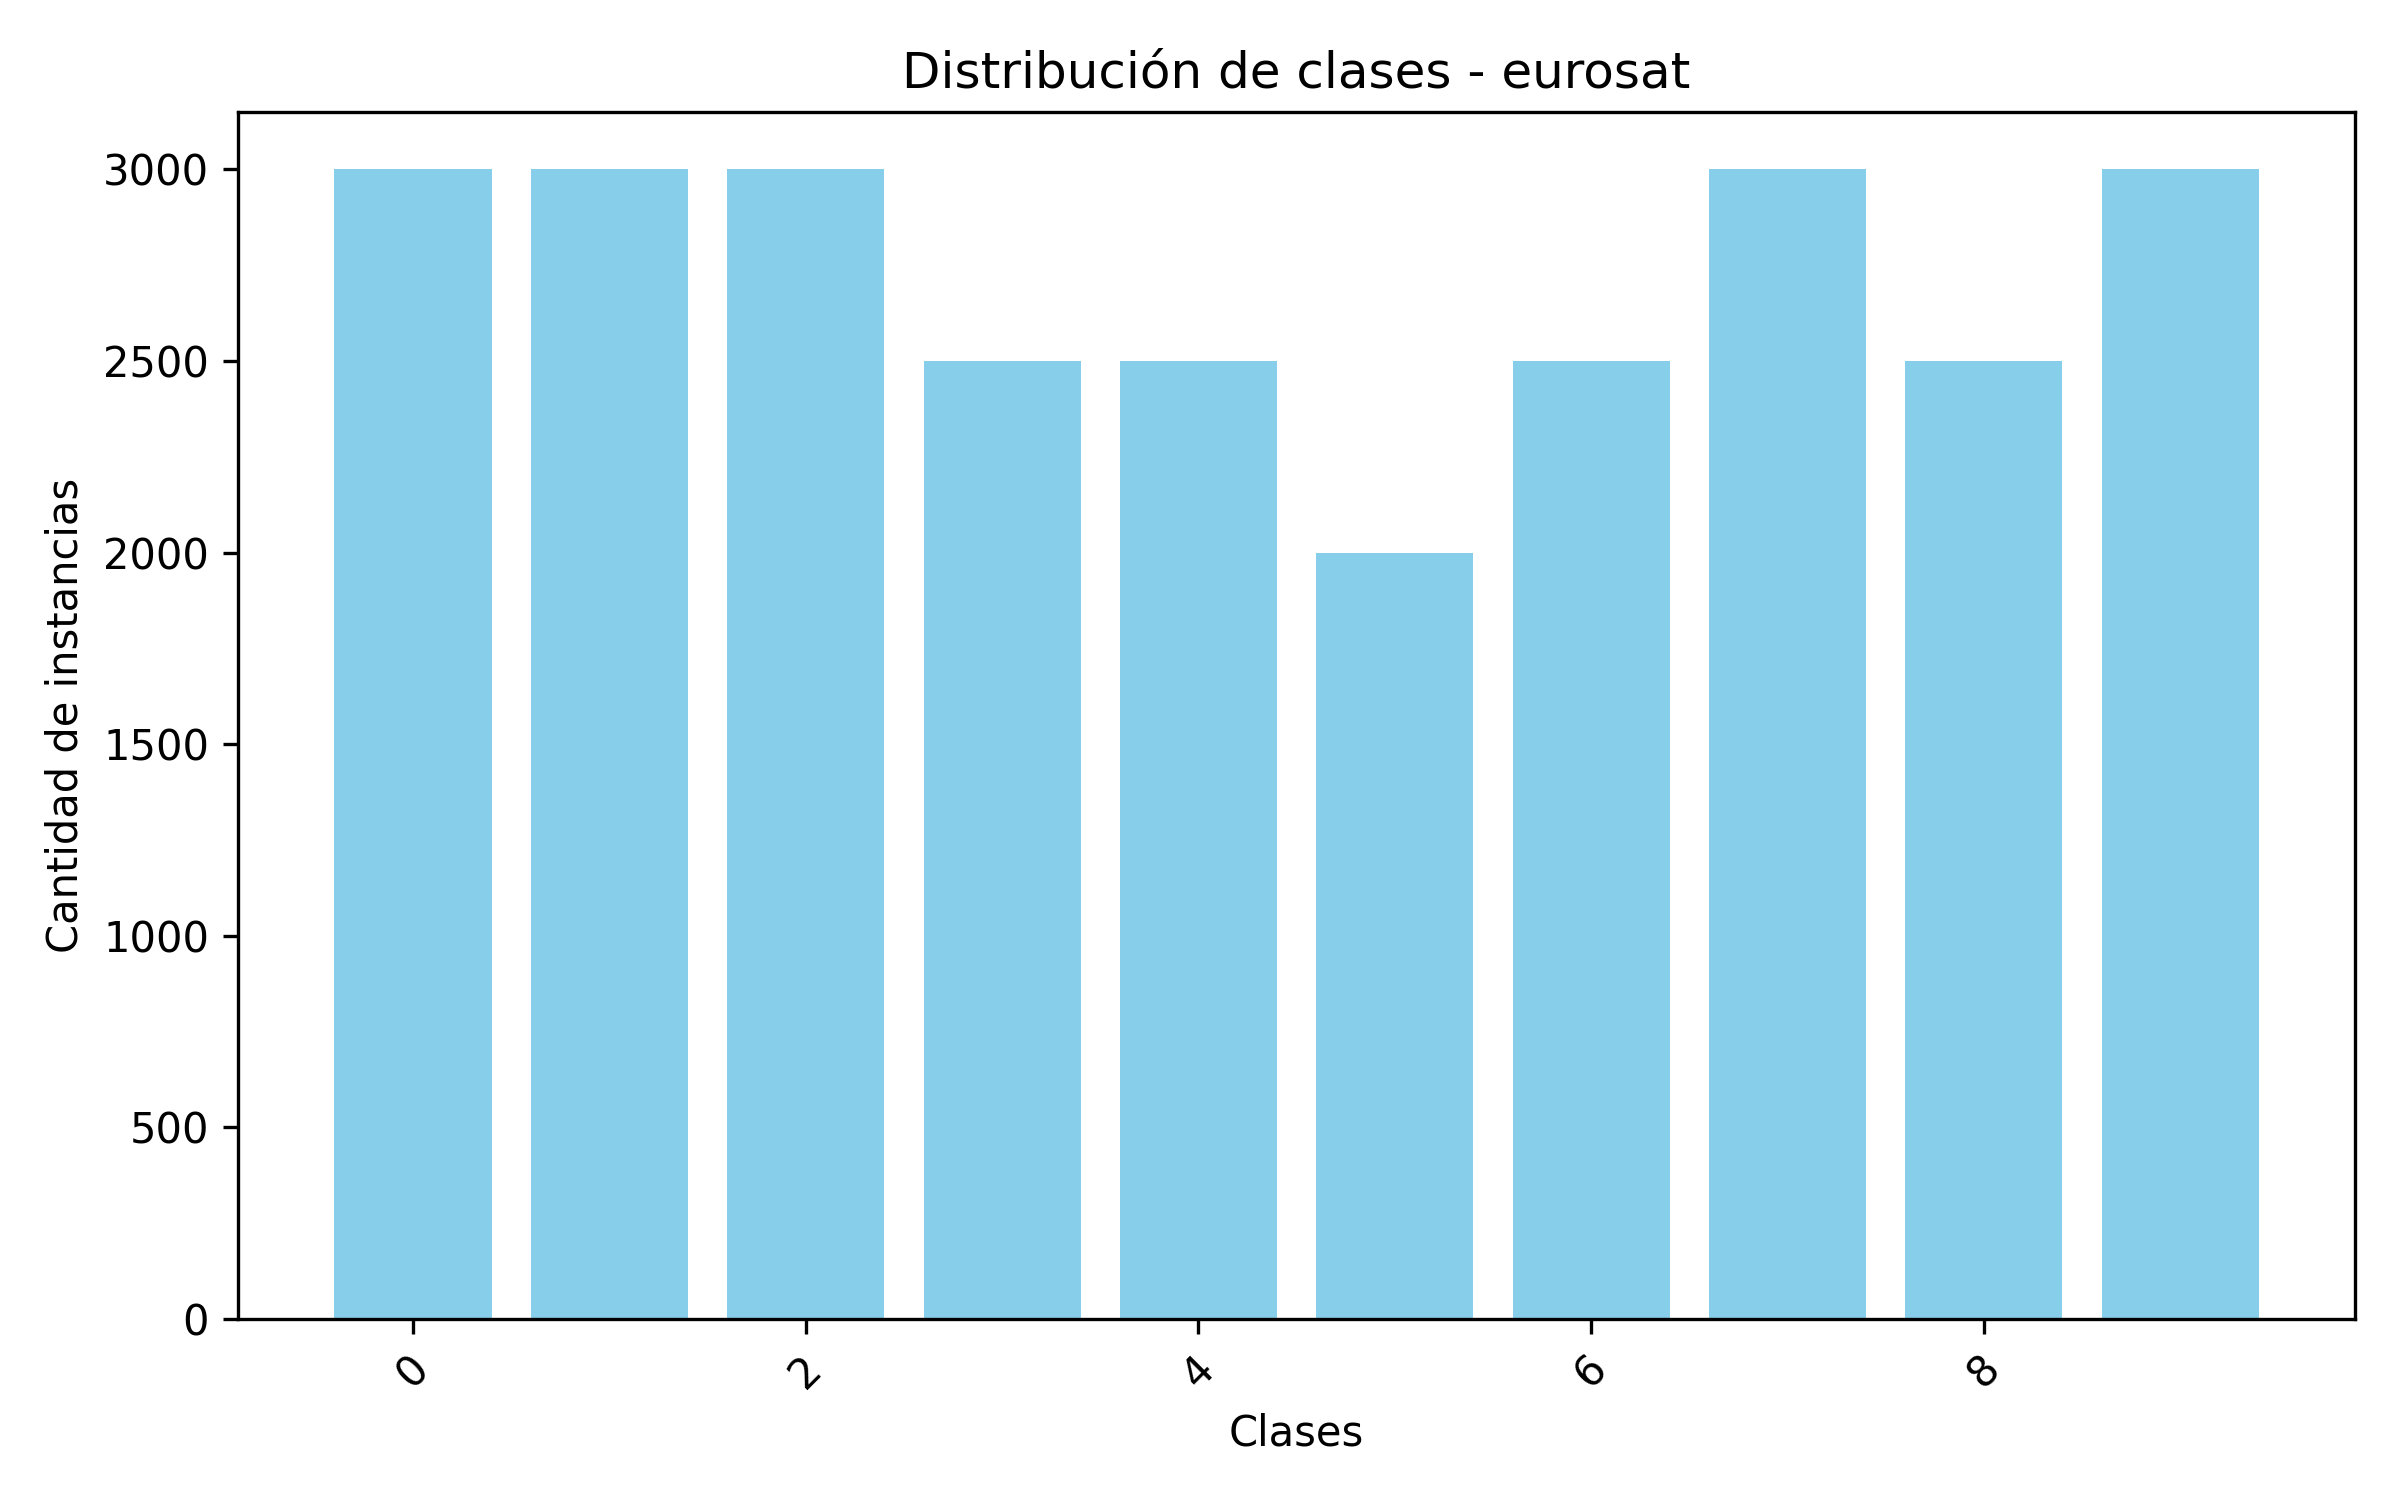
\includegraphics[width=\textwidth]{eurosat_distribucion_2025-07-17_1558.png}
  \caption{EuroSAT}
\end{subfigure}

\caption{Distribución de clases en los datasets utilizados}
\label{fig:distribucion_datasets}
\end{figure}


Se observa que todos los conjuntos presentan algún grado de desbalance, especialmente Ecoli y Glass, donde algunas clases minoritarias representan menos del 5\% del total. Este fenómeno también se replica, aunque en menor medida, en EuroSAT, un dataset multiclase de naturaleza visual (imágenes satelitales), donde la clase menos representada alcanza apenas el 7.4\%.

A continuación se describe brevemente cada uno de los conjuntos utilizados:

\begin{itemize}
    \item \textbf{Breast Cancer (WDBC):} Contiene 569 registros de biopsias mamarias, con 30 atributos que describen características del núcleo celular. El objetivo es clasificar los casos como benignos (B) o malignos (M). La clase minoritaria corresponde a los casos malignos (37.3\%).

    \item \textbf{Ecoli:} Este dataset biológico contiene 336 instancias que describen proteínas y su localización celular en \textit{E. coli}, distribuidas en 8 clases. Presenta un fuerte desbalance, con clases como \texttt{imL} o \texttt{imS} que solo aparecen 2 veces (0.6\%).

    \item \textbf{Glass:} Contiene 214 muestras químicas de vidrios con 9 atributos relacionados a su composición. Las clases representan diferentes tipos de vidrio (ventana flotada, contenedor, etc.). La clase menos representada tiene solo 9 muestras (4.2\%).

    \item \textbf{Heart Disease (Cleveland):} Dataset clínico con 303 instancias y 5 clases que reflejan distintos niveles de presencia de enfermedad cardíaca (0 a 4). La clase minoritaria (nivel 4) representa apenas el 4.3\%.

    \item \textbf{EuroSAT:} Conjunto visual compuesto por 27,000 imágenes RGB satelitales de tamaño $64\times64$ píxeles, distribuidas en 10 clases que representan distintos tipos de cobertura terrestre (bosques, campos de cultivo, zonas urbanas, etc.). Es el dataset más grande y diverso del conjunto experimental, con un desbalance moderado (la clase minoritaria representa el 7.4\%).

\end{itemize}

El análisis de estos desequilibrios guió el diseño de los experimentos, asegurando la aplicación adecuada de técnicas de sobremuestreo para abordar la desproporción entre clases. Además, la diversidad de dominios —biomedicina, bioinformática, química, cardiología e imágenes satelitales— permitió validar la robustez de las técnicas evaluadas en contextos heterogéneos.
